\chapter{Design}
Dette kapitel indeholder en beskrivelse af design valgene for Firebase databasen og applikationen, samt hvordan disse er implementeret. \\

\section{Firebase database}

\section{Applikation}
Til udvikling af applikationen er der brugt et MVC design, som vist herunder, på figur \ref{fig:MVC}
\begin{figure}[H] % (alternativt [H])
	\centering
	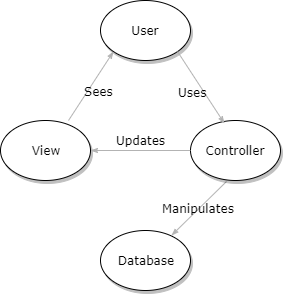
\includegraphics[height=10cm, width=10cm]{../ArkitekturDesign/Design/MVC}
	\caption{MVC design for Rambøll Tilsyn.}
	\label{fig:MVC}
\end{figure}

Model-View-Controller er et design pattern til opbygning af user interfaces. Model er der alt
data ligger. Det er så Controllerens opgave at manipulere det til Viewet. Viewet er det som
ses af brugeren og som der kan interageres med. Hvis brugeren interagerer med applikationen er
det Controllerns opgave at få det ned i Modellen og få kaldt det nye view frem. \\
Der er brugt MVC design pattern til alle views i applikationen.

\section{Login}

\begin{figure}[H] % (alternativt [H])
	\centering
	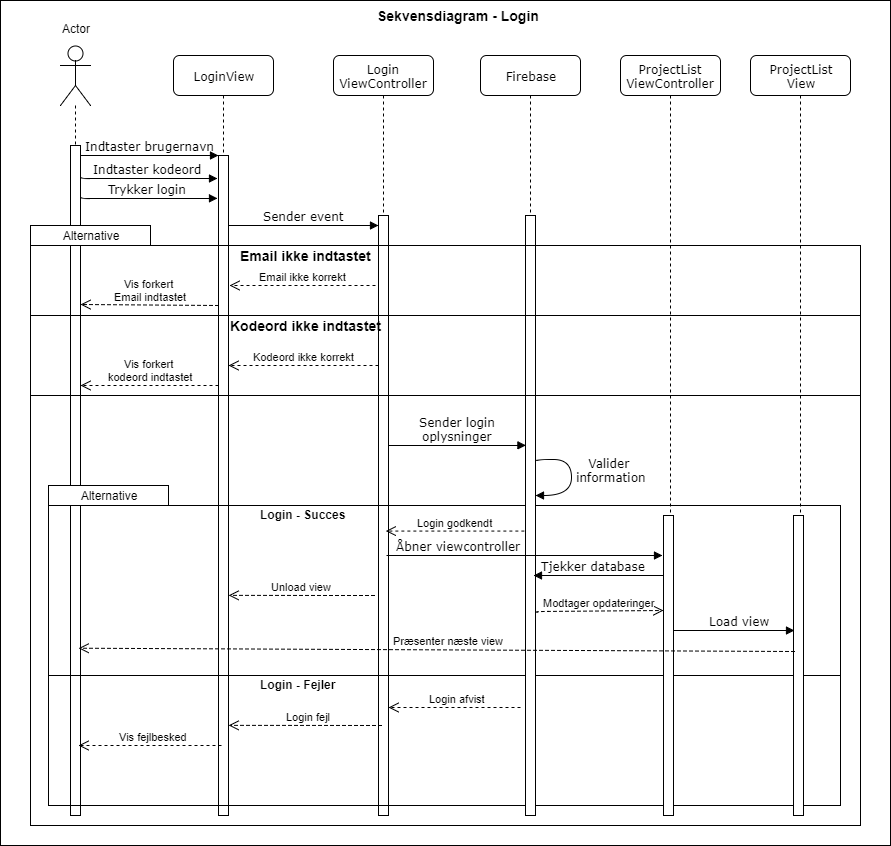
\includegraphics[width=1.1\textwidth]{../ArkitekturDesign/Design/Login/LoginSekvensDiagram}
	\caption{Sekvensdiagram for Login i Rambøll Tilsyn.}
	\label{fig:LoginSekvens}
\end{figure}